
\chapter{Transverse Asymmetry} \label{transv}

\paragraph{}
This chapter is focused on describing the theory behind the \transv. The \transv arises from interference between two scattering amplitudes (the exchange of one and two virtual photons, respectively) and it is deeply connected with the Time-reversal operator. These two scattering amplitude, given by electromagnetic interaction between the incident electron and the nucleus, are explained in this chapter, together with the limits of theory. The chapter ends by presenting the problem of the anomalous observation made by PREX, of zero $A_{n}$ for lead target. In the end we discuss the general formula of $A_{n}$ and we study how the accuracy of a measurement vary increasing the statistics. 

\section{Description of the Process}

The Beam Normal single spin asymmetry, which we will refer for brevity as Transverse asymmetry, originates from the interference of two scattering process. The theory of the electron scattering against a spin $0$ target is extensively treated in \cite{Gorchtein_2008}.
To understand why the interference of this two scattering amplitude give rise to an asymmetry, we first have to look at the kinematic of the experiment:  \newline

\begin{figure}[hbtp]
\centering
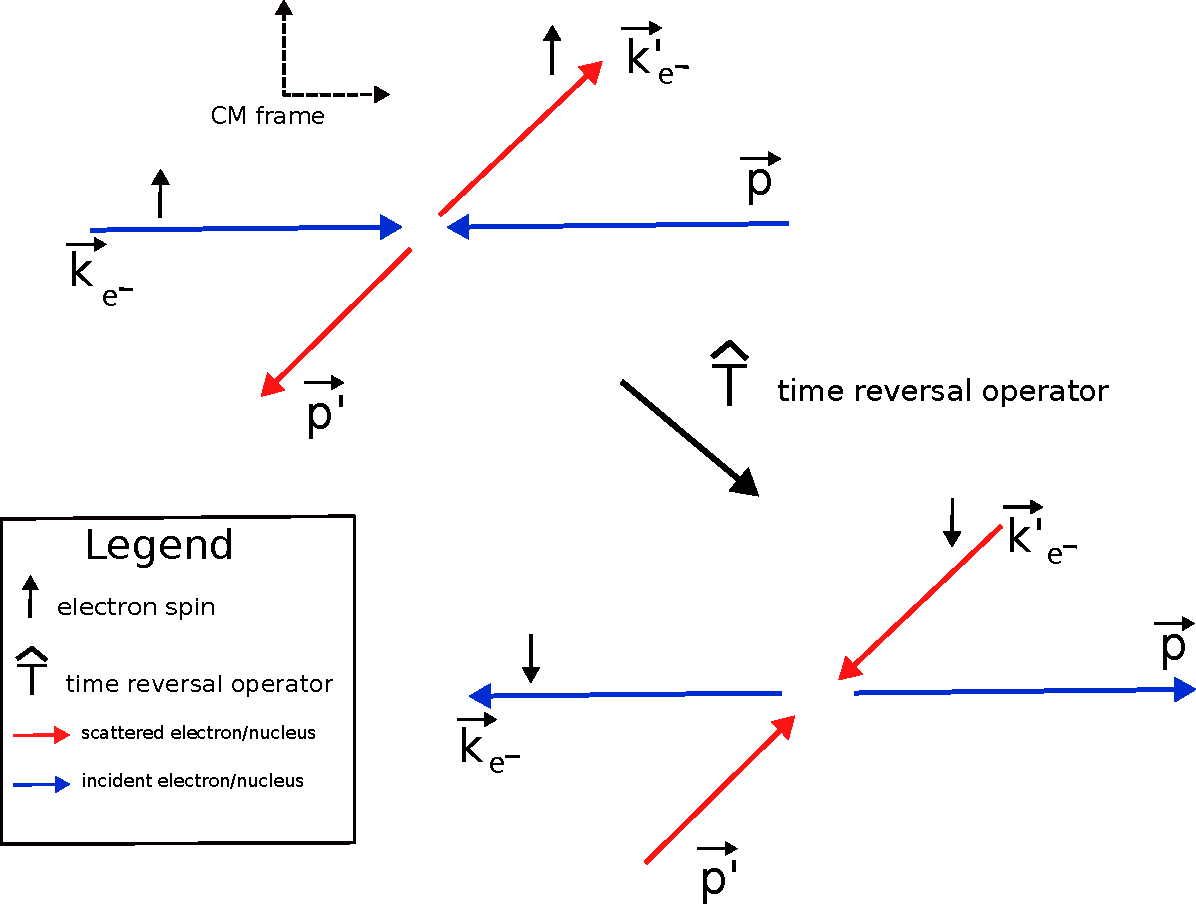
\includegraphics[width = 0.6\textwidth]{Transverse/scattering.pdf}
\caption{Scheme of the scattering process. In blue the incident electron and nucleus, in red the outgoing electron and nucleus. All the quantities are referred to the center of mass frame. The small arrow over the vector represent the electron spin, aligned in the normal plane.}
\end{figure}

Where all the momenta are measured respect to the center of mass frame. In the figure we can confront the two situation before and after applying the Time-reversal operator, $\hat{\Theta}$. Looking at the picture we can understand that : 

\begin{itemize}
\item Before applying $\hat{\Theta}$, we have the incident electron with $\vec{k}$ momenta and the nucleus with $\vec{P}$ momenta, after applying $\hat{\Theta}$ we have that the incident/outgoing electron and the incident/outgoing nucleus are exchanged.
\item The $\hat{\Theta}$ operator acts also on the spin of the electron. Because we are considering process where the spin doesn't flip, the two situations are not equivalent.
\item Considering that the process is elastic, the kinematic is the same, taking $\vec{p}$ and $\vec{k}$ as the initial particle momenta, or $\vec{p}'$ and $\vec{k}'$. 

\end{itemize}

The time-reversal operator seems to connect the two different cases of UP and DOWN polarized electron. Our effort is to measure the asymmetry between the two cross section:

\begin{equation}
A = \frac{\sigma_{\uparrow} - \sigma_{\downarrow}}{\sigma_{\uparrow} + \sigma_{\downarrow}}
\end{equation}

And it's particularly clear that a non-zero asymmetry depends on how the time-reversal act on the elastic amplitude of the process. \\
With this idea, let's see in more detail the $\hat{\Theta}$. We know that $\hat{\Theta}$ is an anti-unitary operator that can be always seen as:

\begin{align*}
\hat{\Theta} = U \cdot K
\end{align*} 
Where $U$ is an unitary operator, while $K$ is the complex conjugation operator that generates the complex conjugate of each coefficient in front of it. If we consider a ket describing a system we have that:

\begin{equation}
Kc \ket{\alpha} = c^{*} K \ket{\alpha}
\end{equation}

Now, let's consider $H$ as the hamiltonian of our system. We want to apply the $\hat{\Theta}$ operator. We can now use the assumption that the hamiltonian consist of two term, which correspond to the two different scattering process. Because of the electromagnetic interaction conserve $CP$, so also $T$ is conserved, we know in advance that each piece of the hamiltonian commute with $\hat{\Theta}$. Now let's see what happen for an hamiltonian which has an imaginary part:

\begin{equation}
H = H_{R} + i H_{Im} \quad ; \quad \hat{\Theta} H \hat{\Theta}^{-1}= \hat{\Theta}H_{R} \hat{\Theta}^{-1} + \hat{\Theta} i H_{Im} \hat{\Theta}^{-1} \Rightarrow H_{R} - i H_{Im} \neq H
\end{equation}

what we understand from these simple calculation is that to give rise to an asymmetry, we expect an imaginary part of the scattering amplitude different from zero.\\
At the $\alpha$ leading order, the two process of the electron-Nucleus scattering that give rise to the asymmetry involve the exchange of one-photon-exchange (OPE) and two-photon-exchange (TPE). The Feynman diagrams that describes the processes are the following: 

\begin{figure}[hbtp]
\[
\feynmandiagram [scale = 1, transform shape][baseline = (h), horizontal = d to j]{
	a [particle = \(e^{-}\)] -- [fermion, thick] c -- [fermion, thick ] f -- [fermion, thick] g [particle = \(e^{-}\)],
	c -- [photon, edge label = \(\gamma\)] d [blob],
	f -- [photon, edge label = \(\gamma\)] j [blob],
	h [particle = \(C^{12}\)]-- d -- [fermion, thick] j -- k [particle = \(C^{12}\)] ,
	};
\qquad \qquad \qquad
\feynmandiagram [scale = 1, transform shape][ vertical = c to d]{
	a [particle = \(e^{-}\)] -- [fermion, thick] c -- [fermion, thick] g [particle = \(e^{-}\)],
	c -- [photon, edge label' = \(\gamma\), momentum = {[arrow style = red]\(k\)}] d [blob],
	h [particle = \(C^{12}\)] -- [fermion, thick] d -- [fermion, thick] j [particle = \(C^{12}\)],
	};
\]
\caption{TPE and OPE diagrams in electron nucleus scattering.}
\label{fig:FeynmannDiagrams}
\end{figure}

The important quantity to compute the cross section is the scattering amplitude. The scattering amplitude is given by the two contributions: the exchange of a single virtual photon $A_{1}$ and the terms given by the two photon exchange $A_{2}$. In general we can write that the total scattering amplitude $S$:

\begin{equation}
S = \dfrac{e^{2}}{Q^{2}} \overline{u}(k') [ \, m_{e} A_{2} + A_{1} \slashed{P} \,] \overline{u}(k)
\end{equation}

Where in this expression $\vec{P} = \frac{\vec{p} + \vec{p}'}{2}$. The second term $A_{1}$ has a simple expression, given by the form factor of the nucleus:

\begin{align*}
A_{1} = 2Z F_{N}(Q^{2})
\end{align*} 

This expression is obtained if we look at the \ref{fig:FeynmannDiagrams}. For the one photon exchange the first vertex connects the incident and scattered electron, whose expression is given by $-ie \gamma^{\mu}$. The second vertex connect the carbon nucleus with the virtual photon. The carbon is threated like as a spin $0$ particle, and the contribution due to the charge density in enshrined in the form factor. The lagrangian term for a vertex of this type is given by the formula: 

\begin{equation}
\Lagr_{interaction} = +ieA_{\mu}(\Phi \partial^{\mu} \Phi^{\dag} - \Phi^{\dag}\partial_{\mu} \Phi)
\end{equation}

For the spin 0 field $\Phi$. This is not the only piece of the lagrangian: there exist another term of interaction, that involves a vertex with four particles which is not of our interest. This interaction term give rise to the Feynmann rule for spin 0 particle, and we have to substitute for this vertex:

\begin{align*}
-ie(p + p')_{\mu}
\end{align*} 

And we recognize, apart from a factor 2, $\slashed{P}$ which multiplies $A_{1}$. The last term is the feynmann propagator for the photon, that give the $\frac{1}{Q^{2}}$ term. This first part of the scattering amplitude is T-even, and it is purely real, so it is the imaginary part of the two photon exchange which give rise to the asymmetry. The expression that connects the amplitude with the \transv is given by:

\begin{equation} \label{eq:integral}
A_{n} = -\frac{m_{e}}{\sqrt{s}} tan \bigl (\frac{\theta_{CM}}{2} \bigl) \dfrac{\Im(A_{2})}{ZF_{N}(Q^{2})}
\end{equation}

Looking at this formula, the theoretical effort to compute the transverse asymmetry is given by the imaginary part of $A_{2}$. The calculation of this quantity is theoretically challenging, due to the fact that at energies of $\simeq \SI{1}{\giga \electronvolt}$ of incident electrons, contributions from intermediate excited states become important. Because of this, the contribution of $A_{2}$ are given by the sum of elastic intermediate state and inelastic terms, which involve hadronic excitations.

\subsection{Hadronic Tensor}

The imaginary part $A_{2}$ is related to the two-photon exchange. To compute this quantity, we have to perform an integration over the internal momenta of the electron $k_{1}$ (see figure \ref{fig:FeynmannDiagrams}). This contribution, following \cite{Gorchtein_2008}, is given by:

\begin{equation}
\Im(A_{2}) = e^{4} \frac{1}{(2\pi)^{2}} \int \dfrac{l_{\mu \nu} \cdot W^{\mu \nu}}{2E_{1} Q_{1}^{2} Q_{2}^{2}} d^{3}\vec{k_{1}}
\end{equation}

Two new terms appear in this expression. The first term is $l_{\mu \nu}$, named leptonic tensor. This term is given computing the Amplitude for the upper part of the diagram, which involve the incident and scattered electron:

\begin{equation}
l_{\mu \nu} = \overline{u}(k') \gamma_{\nu} (\slashed{k}_{1} + m_{e}) \gamma_{\mu} u(k)
\end{equation}

In this expression is immediate to recognize the feynmann rules for fermion vertex. The term $(\slashed{k_{1} + m_{e}})$ comes from the fermion propagator of the internal electron, which is:

\begin{align*}
\dfrac{i(\slashed{p} + m)}{p^{2} + m^{2}}
\end{align*}

The other term is $W^{\mu \nu}$, the hadronic tensor. For the elastic contribution this term is simply given by the feynmann rules for vertex with spin 0 particles, with the proper correction of the form factor, so we can write:

\begin{equation}
W_{\mu \nu} = \pi \delta((p + k - k_{1})^{2} - M^{2}) (2p + q_{1})_{\mu} (2p' + q_{2})_{\nu} \times Z^{2} F_{N}(Q_{1})  F_{N}(Q_{2})
\end{equation}

At this point, one can substitute in the integral above, and compute the contribution of the transverse asymmetry due to the elastic term. This first terms scales with the nuclear charge $Z\alpha$, and this is important for electron scattering with heavy nuclei. However, this mechanism is important in the energy range of few MeV, and has a minor impact, although not negligible, for higher energy, such as the energy of interest for this thesis.
For the inelastic contributions, the structure of the hadronic tensor is different. Realistic estimate are given only for nearly forward scattering angles. The hadronic tensor is given in terms of the structure functions $W_{1,2}$

\begin{equation}
W^{\mu \nu} = 2 \pi W_{1}(\omega^{2},Q_{1}^{2}) \Bigl( -g^{\mu \nu} + \dfrac{P^{\mu}q_{1}^{\nu} +  P^{\nu}q_{2}^{\mu}}{(P \overline{K})} - \dfrac{q_{1} q_{2}}{(P \overline{K})^{2}}P^{\mu}P^{\nu} \Bigl)
\end{equation}

Several assumption are made to threat this new term. The structure function, for forward scattering angles, can be approximated by a function containing the Compton form factor of the nucleus, neglecting some dependence on $Q_{1,2}$ that let to simplify the integral in equation \ref{eq:integral}. It is beyond our scope to go into a detailed description, which can be found in the articles (\cite{Gorchtein_2006}, \cite{Gorchtein_2008}, \cite{Koshchii_2021}). We emphasize however that for the estimation of the inelastic intermediate state, theoretical calculation are affected by the approximation of forward angles and other assumptions due to lack of data in the dependence of some important variables, such as the Compton form factor for carbon 12, the Compton slope parameter and the use of the approximated Callavan-Gross relation. In summary, the theoretical prediction for the \transv are reliable for small scattering angle, that correspond to lower values ​​in transfer momentum $Q$; the experimental data measure by PREX \cite{HAPPEX:2012fud} for $^{1}H$, $^{4}He$, and $^{12}C$ at $Q$ values of $\SI{0.31}{\giga \electronvolt}$, $\SI{0.28}{\giga \electronvolt}$ and $\SI{0.1}{\giga \electronvolt}$, respectively, are in agreement with the theoretical prediction. The measurement performed at MAMI for $^{12}C$ \cite{Esser:2018vdp} are with higher values of transfer momentum ($Q = \SI{0.2}{\giga \electronvolt}$) and shows a discrete agreement with the theoretical prediction, considering also the systematic uncertainties associated to the poorly known Compton slope parameter.
While the theory presented so far is quite successful in describing the data, it fails completely with $^{208}Pb$. PREX report for lead $0$ asymmetry. This strictly disagreement, although remove the presence of systematic effects due to the BNSSA for PV experiment, suggest to repeat the measure, besides being a theoretical challenge. Also for this reason, after the measurement with carbon, a new measurement of the transverse asymmetry with lead is scheduled.

\begin{figure}[hbtp]
\centering
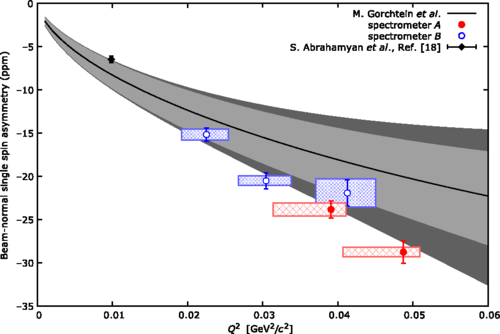
\includegraphics[scale = 0.5]{Transverse/medium.png}
\caption{Transverse asymmetry measured at MAMI for $^{12}C$ target \cite{Esser:2018vdp}. Theoretical calculation for $E_{beam} = \SI{570}{\mega \electronvolt}$  is shown.}
\end{figure}

  

\subsection{Model Description}
\commento{Present the theoretical formula for the Transverse asymmetry, and comment on energy, Z, Z/A depencencies adding together the elastic and inelastic contributions, we end with the following formula which describes the process \cite{PhysRevLett.121.022503}:}\medskip

\begin{equation}
A_{N} = C_{0} \cdot log(\dfrac{Q^{2}}{m_{e}^{2} c^{2}}) \dfrac{F_{Compton}(Q^{2})}{F_{ch}(Q^{2})}
\end{equation}

\section{State of the Experiment}

We have seen so far how the Transverse Asymmetry is related to the interference between two scattering amplitude, and the theoretical model used to describe the process. The goal from an experimental point of view is to measure this quantity. The challenge is to obtain a valid measure of $A_{n}$, which is of the order of $20$ part per million (ppm), taking into consideration all the possible effects that can interfere. To measure $A_{n}$, the straightforward method is to prepare an electron beam, with polarized electron, and send it to a fixed target. The scattered electrons are then collected by a detector placed at a certain angle, and now it's possible to obtain the transverse asymmetry applying the formula:

\begin{equation}
A_{N} (Q,p) = \dfrac{N_{\uparrow}(Q) - N_{\downarrow}(Q)}{N_{\uparrow}(Q) + N_{\downarrow}(Q)} \cdot (\frac{1}{p})   
\end{equation} 

where we have explained the dependence on the transmitted impulse, on the degree of polarization of the beam.
In an experiment of this type, several requests are necessary to have an effective data acquisition:

\begin{itemize}
\item The accelerator must produce a polarized beam, stable over the time, with an high polarization percentage, in order to amplify the effect.
\item The Beam energy needs to be quite stable, and should not depend on the Polarization state of the electrons. A change in the Beam energy associated with the polarization state, can lead to a different count rate for $N_{\uparrow}$ and $N_{\downarrow}$, would make a contribution that would be added to that of the physical process
\item The beam must be correctly aligned with the target, and stable. Again if the position of the target changes according to the polarization of the electrons, it will produce another contribution to the total asymmetry.
\item The beam current should not depend on the polarization state of the electrons. If the beam source depends on the polarization, we will have a difference in the event rate and then another false asymmetry.
\item it's necessary to reject possible double elastic scattering events, which may contribute to the total asymmetry. 
\end{itemize}

All this demands can be satisfied with an accelerator that has stabilization devices with great precision and that can sustain high beam intensities. This last request is necessary to accumulate enough statistics to measure the transverse asymmetry with an accuracy about 1 ppm, in view of the future PV experiments. We can quantify how the statistical error varies according to the amount of data available. With the assumption that $N_{\uparrow,\downarrow}$ are gaussian distributed variables, we can compute the expected variance

\begin{equation}
Var[A_{n}] = \dfrac{1 - A^{2}}{N_{\uparrow} + N_{\downarrow}} 
\end{equation}

For a single measurement of the $A_{n}$. For multiple measurement $n$, the variance scales as $\frac{1}{n}$.
Because $A_{n}$ is expected to be smaller respect to 1, we can approximate the above formula:
\begin{equation} 
V[A_{n}] = \dfrac{1}{2N \cdot n}  \label{eq:Error}
\end{equation}

The error associated to the reconstructed asymmetry is the square root of the above quantity. If we impose that the error must be $\le 1ppm$ we can easily obtain that the quantity $n\cdot N$:

\begin{align*}
n\cdot N \le \frac{1}{2} \cdot 10^{12}
\end{align*} 

We will see later that achievable rates $N_{\uparrow,\downarrow}$ are in the range (20000,60000) counts per event for a carbon target. This number can not be increased at will by acting on the beam current. The first reason is oblivious: the beam source can produce only a certain amount of electrons before loosing, furthermore a beam with great intensity for an extended periods of time can damage the carbon target up to the risk of melting it. 
Another idea might be to increase the thickness of the target, to take advantage of the larger cross section. However this does not take into account that by doing so the number of double scattering event is increased. To avoid this the scientific community that deals with these nuclear physics measurements respect the convention that the target thickness should be less than the $10 \%$ of the radiation length of the material.
